\documentclass[tikz, border=10pt]{standalone}
%\documentclass[a4paper,12pt]{article}

\input{Preambulo.tex}
\input{Auxiliar.tex}

\begin{document}

\thispagestyle{empty}

    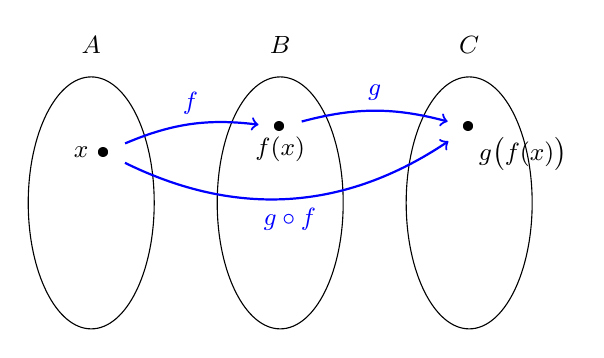
\begin{tikzpicture}[scale=0.8, every node/.style={font=\small}]
    % Conjuntos A, B e C
    \draw (0,1.5) ellipse (1 and 2);
    \draw (3,1.5) ellipse (1 and 2);
    \draw (6,1.5) ellipse (1 and 2);
    \node at (0,4) {\(A\)};
    \node at (3,4) {\(B\)};
    \node at (6,4) {\(C\)};

    % Elementos
    \node (x) at (0.2,2.3) {\textbullet}; 
    \node[left=2pt] at (x) {\(x\)};
    \node (fx) at (3,2.7) {\textbullet}; 
    \node[below] at (fx) {\(f(x)\)};
    \node (gfx) at (6,2.7) {\textbullet}; 
    \node[below right] at (gfx) {\(g\big(f(x)\big)\)};

    % Setas com função e ajuste das pontas
    \draw[->, thick, blue, shorten >=2pt, shorten <=2pt] 
        (x) to[bend left=15] node[midway, above] {\(f\)} (fx);
    \draw[->, thick, blue, shorten >=2pt, shorten <=2pt] 
        (fx) to[bend left=15] node[midway, above] {\(g\)} (gfx);
    \draw[->, thick, blue, shorten >=2pt, shorten <=2pt] 
        (x) to[bend left=-30] node[midway, below] {\(g \circ f\)} (gfx);
\end{tikzpicture}

\end{document}

#Como compilar e gerar uma imagem svg (Scalable Vector Graphics) para colocar em html
#pdflatex EsbocoTikz.tex
#pdf2svg EsbocoTikz.pdf EsbocoTikz.svg
